\chapter{Simulations}\label{chap:simulations}
In this chapter, we describe the setup and execution of the simulations used to evaluate the load balancing protocols. Simulations are conducted using the PeerSim simulation tool for Java. Different topologies are implemented. For every simulation a output file is generated containing, the loads, sums and weights of every node per round and the mean squared error of the graph per round. Also the output files contain information regarding the setting of the simulation, like the network size or the topology chosen for the simulation. These output files are processed and analyzed using Python, with \textit{Matplotlib}, as it provides a variety of options for plotting and a comprehensive and detailed documentation.

\section{PeerSim}
PeerSim is a simulation tool developed for the Java programming language. PeerSim is composed of two engines: the event-driven engine and the cycle-driven engine. We chose the cycle-driven engine for our simulations. PeerSim is specifically designed for large-scale network simulations due to its high scalability and the ability to program with pluggable components. A PeerSim simulation generally follows four main steps:
\begin{enumerate}
    \item \textbf{configuration file creation}: The simulation begins with the creation of a configuration file that defines the simulation parameters. This file specifies the network size, the protocols to be used, and other necessary settings.
    \item \textbf{protocol selection}: After the configuration step, the next step is to choose the protocol or protocols to be simulated. This can involve running multiple protocols in parallel or focusing on a single protocol.
    \item \textbf{control object selection}: Now, it is time to initialize control objects to monitor simulation parameters. Our control objects are classes named \textit{<Protocol>Observer}.
    \item \textbf{simulator class invoking}: Lastly, the configuration file has to be invoked by the \textit{peersim.Simulator class} \cite{peersimdocs}. For that, the IDE is instructed to call the simulator class on click of the "run"-button. Alternatively, a command line in the terminal can also invoke the simulator class. More on this in the PeerSim documentation.
\end{enumerate}
PeerSim provides many classes and interfaces for simulation. For the cycle-driven approach a interface \textit{CDProtocol} is provided by the simulation framework, which implements the \textit{nextCycle} method. The \textit{nextCycle} method is executed in the beginning of every round.

Nodes in PeerSim are implemented as containers that hold various protocols. Every node is identified by an ID and interacts with the \textit{Linkable} interface, which provides 
access to the neighboring protocols. A class that implements the \textit{Linkable} interface, allows overwriting different methods, like the \textit{getNeighbor} method, which retrieves a neighbor with a specified ID. The \textit{degree} method, returns the number of connections a node has. A method \textit{addNeighbor}, adds a neighbor to a node's set of neighbors. To monitor and modify the simulations control objects are required. A class implementing the \textit{Control} interface includes the \textit{execute} method. This method can be used to observe or alter the simulation at each round \cite{peersimdocs}.

\section{Implementation Details}
Both implementations of the protocols are composed of at least two different java classes: an observer class and a protocol class. Additionally, a shared parameter class, named \textit{LoadBalancingParameters.java}, is utilized by all protocols for storing shared parameters (e.g. the round number or the dimensions of specific graphs). Protocol-specific parameters are managed within their respective protocol classes. The observer class of a protocol handles the implementation and the monitoring of the protocols. The implementation of the topologies is also handled in the observer classes. To generate a link between two nodes, we simply add the node ID to the node's set of neighbors. Since we are in a static setting, the links are created during round 0, which is dedicated to initialization tasks. The output files are generated on-the-fly, while simulating. At the end of each round the mean squared error values are appended to the output file.

\begin{figure}[H]
    \centering
    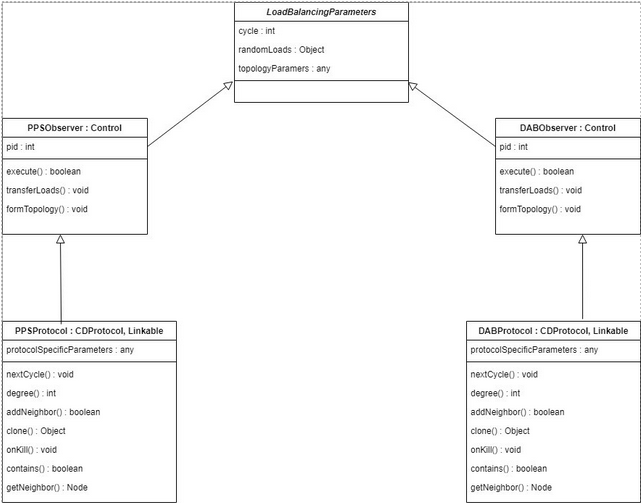
\includegraphics[scale=0.7]{figures/uml/projectArchUml.png}
    \caption{project structure}
    \label{fig:uml}
\end{figure}
